\section{Scene and object recognition with Computer Vision}

\begin{frame}
\frametitle{Tool detection \& pose estimation}
\begin{columns}
\column{0.65\textwidth}
\begin{center}
\begin{figure}[!htb]
\centering
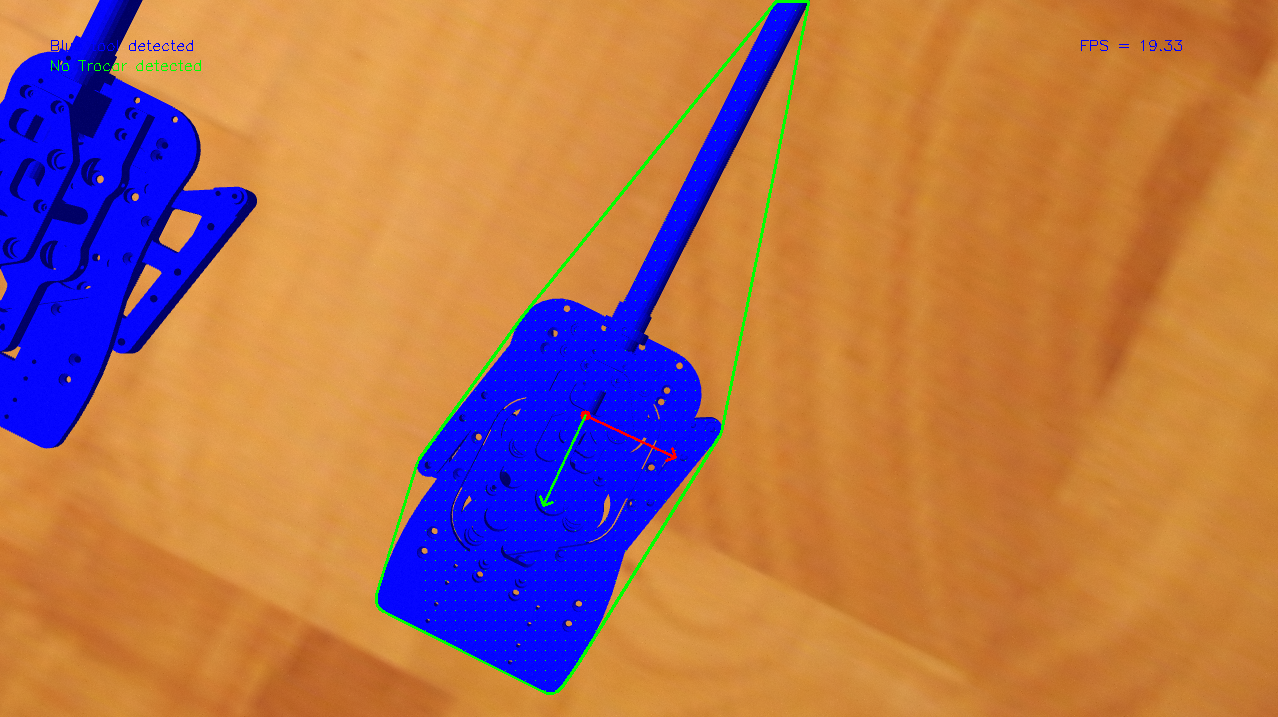
\includegraphics[width=\textwidth]{../images/tool-pose.png}\\
\caption{Tool's ROI, convex hull, center of mass and orientation vectors}
\end{figure}

\end{center}


\column{0.35\textwidth}
$\mathbf{a},\mathbf{b}$: orientation vectors, solutions of
\[
\mathbf{C} \mathbf{v} = λ \mathbf{v}
\]
\[
\mathbf{C} = \begin{bmatrix}
σ(x,x) & σ(x,y) \\
σ(y,x) & σ(y,y) \\
\end{bmatrix}
\]
\end{columns}

\begin{columns}
\column{0.5\textwidth}
\[
\left( \bar{x}, \bar{y} \right) = \left( \frac{1}{N}\sum_{i=1}^{N} x_i , \frac{1}{N}\sum_{i=1}^{N} y_i \right)
\]
\column{0.5\textwidth}
\[
σ(x,y) = \frac{1}{n-1} \sum_{i=1}^{N} ( x_i - \bar{x} )( y_i - \bar{y} )
\]
\end{columns}
\end{frame}


\begin{frame}
\frametitle{Calculation of grasping points}
\begin{center}
\begin{figure}[!htb]
\centering
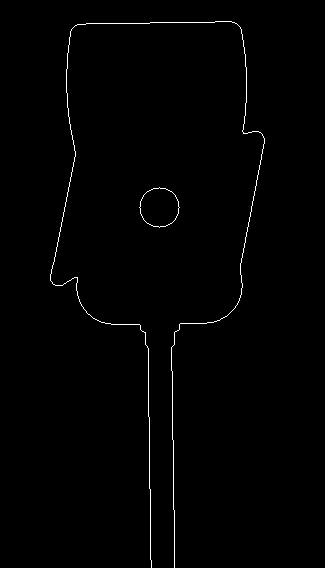
\includegraphics[width=0.15\textwidth]{../images/grasp_points_1.png}
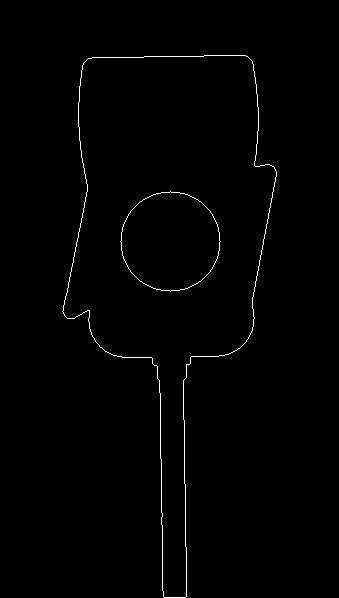
\includegraphics[width=0.15\textwidth]{../images/grasp_points_2.png}
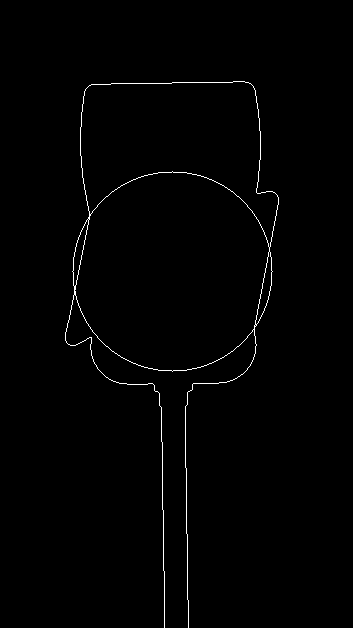
\includegraphics[width=0.15\textwidth]{../images/grasp_points_3.png}\\
\caption{Finding candidate grasping points from the intersections of a growing circle mask $I_1(x,y)$ and the contour of the detected surgical tool $I_2(x,y)$}
\end{figure}

\begin{enumerate}
\item $\mathbb{G} = \underset{(x,y)}{\arg\max} I_1(x,y) \odot I_2(x,y)$
\item match points with stereo 3d points
\item check feasibility with gripper kinematics
\end{enumerate}

\end{center}
\end{frame}
